%---------- Inleiding ---------------------------------------------------------

\section{Introduction}
\label{proposal-sec:proposal-introduction}

Jump rope is an evolving sport.
Year after year, an increasing amount of high-level competitors are pushing the limits of jump rope.
% TODO : source?
This results in new skills, new combinations, better physiques, better rope material, and faster movements. For the judges to keep up with the jumpers and to correctly assess scores to a routine, Double Dutch freestyles\footnote{Two turners, with one or more jumpers} are reviewed at half speed in International competitions or even at nationals in Belgium.

Head judges around the world question the best way to judge athletes correctly so as to give an accurate and objective ranking in national or international competitions.
Many solutions have been provided: another judging rule set\footnote{The current rule set is enforced and maintained by \href{https://www.gymfed.be/}{Gymfed}, closely related to the international judging-rules from the \href{https://ijru.sport/}{International Jump Rope Union}}, splitting judge responsibility, replaying the routine at half speed \dots

However, with the increasing popularity of image recognition, more powerful computers, applications that recognize objects in images \autocite{Singh_Gill_2022}, implementations detecting simple human actions \autocite{LUQMAN_2022}, examples of action recognition in other sports \autocite{Yin_2024} and the successful test of \href{https://nextjump.app/}{NextJump}'s AI speed-counter, head jurors wondered about the possibility of using modern technologies like artificial intelligence to improve the judging results of jump rope freestyles.

This results some in the main research question of this paper: \textbf{``How can artificial intelligence be incorporated into jump rope freestyles to increase the objectiveness and accuracy of judging?''}.

\subsection{Problem domain}
\label{proposal-subsec:proposal-intro-problem-domain}

Jump rope, like gymnastics or athletics, exists in many disciplines like Speed, Single Rope freestyle (single/pair/team), Chinese Wheel (CW) or Double Dutch (single/pair).
To accurately judge routines, each discipline has its own rules. Although interlapped, differences exist. Each athlete or team then performs a choreography of 60 to 75 seconds showcasing their favorite skills and uniqueness.

\subsubsection{What are the challenges for judges today?}
\label{proposal-subsubsec:proposal-intro-question-challenges-for-judges}

On competitions, judges watch the routine live to annotate the difficulty or creativity. Each judge then pays attention to his assigned part, e.g. movement, musicality or difficulty, all of those elements contributing to the total score of the freestyle. The main problem now is for judges to keep up with double dutch routines. Single rope freestyles are still manageable. To increase the accuracy, difficulty-certified judges \footnote{Those judges judging the difficulty of double dutch routines.} are already allowed to review freestyles at half speed in order to score them accurately.

\subsubsection{How is difficulty scored?}
\label{proposal-subsubsec:proposal-intro-question-difficulty-scored}

Performed skills each have a level, which will be written down when seen by the judge. Each level also has a numeric score that contributes to the total difficulty of the routine. Judges see and calculate/memorize the level of each skill, write it down, count the number of levels jumped and calculate the diff score.

\subsubsection{What are the skills and transitions that need to be recognized?}
\label{proposal-subsubsec:proposal-intro-question-what-are-the-skill}

% TODO : provide examples of skills
For double dutch, there are two turners and at least one jumper. All three of them act as a unit and execute skills or turner combinations. Jumpers can do a handstand, push-up or a cartwheel, while turners can turn with their arms crossed, on the back or rotating two ropes underneath the jumper at once. Furthermore, combining skills of a jumper while doing a special rotation contributes to more difficulty and more points. Even different transitions like a turntable, which is a push-up to a push-up while your body position changes a quarter is a different transition.


% TODO : omit or shift
%\subsubsection{What can be done to increase the accuracy of judging?}
%\label{proposal-subsubsec:intro-question-how-to-increase-accuracy}

% The preferred solution in this proposal is an AI-model recognizing (sub)skills and transitions in a double dutch single freestyle (DD3) as assigning correct levels at world championships or even nationals in Belgium is perceived to be hard and the current main issue.


\subsection{Solution domain}
\label{proposal-subsec:proposal-intro-solution-domain}

Until now, only the scope has been narrowed down. The focus will be put on double dutch freestyles. Getting to know the topic is great, but this doesn't get us further into the solution. Let's jump into it.

% TODO : update order
\subsubsection{Which modern technologies can be used to increase score accuracy of jump rope freestyles}
\label{proposal-subsubsec:proposal-intro-question-integration}

As reviewing routines at half speed still has his limits, using machine learning (an AI-model) could reduce time spent on judging routines. The idea would be a machine learning model recognizing (sub)skills and transitions in a double dutch single freestyle. (DD3)

\subsubsection{Which data is available for the machine learning model to use?}
\label{proposal-subsubsec:proposal-intro-question-data}

To recognize hundreds of skills, variations and transitions, lots of data is needed. Both individual and team freestyles are mostly recorded by clubs themselves or event organizers, some which are available on social media. The task is to explore and gather as much as possible.

\subsubsection{When are predictions acceptable to potentially use on competitions?}
\label{proposal-subsubsec:proposal-intro-question-acceptable-results}

Judges do make mistakes, just like the machine learning models, but we do need a baseline for acceptable results. Past competition scores can be used to define a target.

\subsubsection{How can the AI-judge as a hybrid model increasing judge quality of the judges?}
\label{proposal-subsubsec:proposal-intro-question-hybrid-model-judge-quality}
Can the AI-judge \footnote{The machine learning model predicting performed skills} be used to train new judges or brush up the knowledge of current judges? Meanwhile, can they verify the predicted labels by the model to use as new training data?

\subsubsection{Which activity recognition examples can be used or altered as a base guidance?}
\label{proposal-subsubsec:proposal-intro-question-earlier-research-guidance}

Quick searches give examples of object recognition \autocite{Diwaker_2022}, detecting sign language \autocite{Bora_2023} or activity recognition (e.g. the kinetics dataset - riding a bike, reading a book, playing an instrument \autocite{Kay_2017}).
These implementations can be used as a first guide.
Those examples give the idea that data mostly seem more to be centered, which is not the case in jump rope videos, a solution needs to be found for that. The second problem is that freestyles can consist of more than fifty different skills, which takes a long time to cut manually.


\subsubsection{What would be a minimal Proof of Concept (PoC)?}
\label{proposal-subsubsec:proposal-intro-question-poc}

The PoC would be a model recognizing the most common skills and transitions.
This could mean omitting or just marking special combinations, longer double dutch switches or long time sequences of emptiness in general. Preferably, the PoC should be able to generalize uncommon skills that are still definable as normal. Better described would be knocking on the door three times, someone's at the door, but knocking four times or with a bonk in between is also recognizable \footnote{See specified example in section \ref{proposal-subsec:literature-unknown-unusual-skills}} for a more concrete case.

\subsubsection{How much data is expected to increase the accuracy off the Judge?}
\label{proposal-subsubsec:proposal-intro-question-expected-data-to-increase-accuracy}

The amount of videos will keep rising, but will the current amount be sufficient? If it's not enough, how much more would be expected and what about uncommon skills. Do we need to specially record them? But what about new skills on competitions?

\subsection{Additional questions}
\label{proposal-subsubsec:proposal-intro-question-additional}

The proof of concept will probably raise a lot of questions as a byproduct such as:

\begin{itemize}
    \item How can we use the AI-Judge to improve judges?
    \item What needs to change on a working model, to apply it on other judge-related sports such as gymnastics, synchronized swimming, figure skating \dots
\end{itemize}


\subsection{Introduction summary}
\label{proposal-subsubsec:proposal-intro-summary}

With some general knowledge about jump rope and thethesis goal defined, further research, (label)definitions, model selection, and implementation can be performed.
Let’s start by exploring earlier work while slowly increasing the number of jump rope definitions.


%---------- Background information ---------------------------------------------------

\section{Literature review}%
\label{proposal-sec:literature}

% TODO: (Check order)

The research towards skill-recognition will be done by steps. First will be an introduction of skills, after which computer vision will be explored along with NextJump's speed-counter. With a general proposed flow in mind, enables an improved research towards specific models and fine-tuning of the expected approach and potential challenges to recognize skills.

\subsection{Skills intro}
\label{proposal-subsec:literature-basisskills}

Earlier we described the presence of multiple disciplines in Jump Rope. To keep the research doable, skill recognition will be started for one discipline, namely DD3 freestyles, which already contains some Chinese wheel integration.

\subsubsection{Double Dutch Single Freestyle - DD3}
\label{proposal-subsubsec:literature-dd3}

% TODO : add DD figure for clarification
DD3 consists of two turners and one jumper alternating ropes. Elements in Double Dutch are similar to single rope, but different at the same time. The jumper does all the skills, mainly powers, gymnastics or footwork, since he doesn't need to hold the rope. Turners can manipulate the rope using multiple unders, turner-skills like crossed arms, EB, toad\dots or even involve gymnastics themselves.
To judge double dutch, `snapshots` are taken, then the corresponding level will be given depending on the combination of turners, skills and rope-rotations.

Like any discipline, mistakes can happen, they'll be deducted from the total score.

Some examples with their current corresponding levels in double dutch.

% TODO : bijlage bij BP?
\begin{itemize}
    \item Powers
    \begin{itemize}
        \item push-up - to plank position and pushing upwards while pulling the rope underneath your feet. (lvl 2)
        \item split (2)
        \item frog - handstand (2)
        \item swift/V-kick (3)
    \end{itemize}
    \item Gymnastics
    \begin{itemize}
        \item cartwheel (2)
        \item kip (3)
        \item salto (4)
    \end{itemize}
    \item Turners
    \begin{itemize}
        \item cross (c - crossed arms on the stomach) (+2/+0)
        \item crouger (raise knee, put your arm underneath it) (+1)
        \item EB (arm on stomach + arm on back) (+1)
        \item TS (arms crossed behind the back) (+1/+1)
    \end{itemize}
    \item Multiples
    \begin{itemize}
        \item double - DU - 2 rotations (+1)
        \item triple - TU - 3 rotations (+2)
        \item quad - QU - 4 rotations (+2)
        \item quint - 5 rotations (+3)
    \end{itemize}
\end{itemize}

Each power can then be varied one handed, as a turntable, as a consecutive \dots, which gains extra levels. Judges calculate or memorize the whole level of each skill/transition. Without further context, annotations like (+1/+1) can already seem confusing, well it is.



\subsection{Challenges of judging}
\label{proposal-subsubsec:literature-judge-challenges}

\begin{table*}[]
    \begin{tabular}{lllllllll}
        Year & World & Europe & Belgium & Usa   & Hungary & Germany & China \\
        1998 &       &        &         &       &         &         &       \\
        1999 & 80    &        & 80      &       &         &         &       \\
        2012 &       &        &         &       &         &         &       \\
        2015 &       &        &         &       &         &         &       \\
        2016 & 111   & 103    &         &       &         & 103     &       \\
        2019 & 111   &        & 102     & 105.5 &         &         &       \\
        2020 & 111   &        & 102     & 105.5 &         &         &       \\
        2021 & 111   &        & 103.5   & 105.5 &         &         &       \\
        2022 & 111   &        & 103.5   & 105.5 &         &         &       \\
        2023 & 113   &        & 103.5   & 106   &         &         & 113   \\
        2024 & 113   & 108    & 103.5   & 106   &         &         & 113
    \end{tabular}
    \caption{History of speed records males}
    \label{proposal-tbl:speed-records-male}
\end{table*}

\begin{table*}[]
    \begin{tabular}{lllllllll}
        Year & World & Europe & Belgium & Usa   & Hungary & Germany & China \\
        1998 & 83    &        &         &       & 83      &         &       \\
        1999 &       &        &         &       &         &         &       \\
        2012 &       &        & 102     &       &         &         &       \\
        2015 & 105   & 105    &         &       & 105     &         &       \\
        2016 & 105   & 105    & 102     &       & 105     &         &       \\
        2019 & 108.5 & 105    & 102     & 100.5 & 105     &         & 108.5 \\
        2020 & 108.5 & 105    & 102     & 100.5 & 105     &         & 108.5 \\
        2021 & 108.5 & 105    & 102     & 100.5 & 105     &         & 108.5 \\
        2022 & 108.5 & 105    & 102     & 100.5 & 105     &         & 108.5 \\
        2023 & 108.5 & 105    & 102     & 100.5 & 105     &         & 108.5 \\
        2024 & 108.5 & 105    & 102     & 100.5 & 105     &         & 108.5
    \end{tabular}
    \caption{History of speed records females}
    \label{proposal-tbl:speed-records-female}
\end{table*}

As introduced earlier, based on own experiences and statements of colleagues, the sport is evolving. These statements are supported by commentary from the IJRU world championship livestream day 1 \autocite{IJRU_yt_2023_livestream_day1} to day 8 \autocite{IJRU_yt_2023_livestream_day8}.
Speed records are slowly rising, see table \ref{proposal-tbl:speed-records-male} or \ref{proposal-tbl:speed-records-female} \footnote{\autocite{www_speed_30s_1999_WORLD}, \autocite{www_speed_30s_2024_BE}, \autocite{www_speed_30s_2024_IJRU_WORLD}, \autocite{www_speed_30s_2024_USA_AMJRF}}, also quads or quints in single rope freestyles are becoming the norm, where 10 to 15 years ago, it was considered a wow factor. This is also the case for double dutch; more variations, more turner involvements, faster and longer skill-sequences etc.
All which need to be perceived using the same old brain capacity of a judge.
To help judges and improve, some actions already took place.

\subsubsection{Splitting responsibility}
With the current rules, judges are devided in two main categories, those judging difficulty and those judging creativity. Creativity is further split into execution, entertainment, musicality and variation. This breakdown allows increased attention on different aspects of a routine, thus decreasing potential observation mistakes.

\subsubsection{Multiple panels}
Using two ormore judge-panels, more freestyles can be evaluated at the same time. While one
panel is watching a freestyle, the other can summarize and calculate the total score. Having the same panel judge the same category, e.g. juniors vs seniors, also decreases the effect of differences as a people between judges, e.g. being more strict, less observational moment(s), incorrectly memorized a skill-level etc.

\subsubsection{Adapting the rules}
Changing the rules about how a freestyle must be evaluate, can impact the way of thinking, memorizing or calculating the level, score or deduction of a skill. This was tried by using the current 'snapshot' system for double dutch. This was still perceived as hard based on reactions of fellow exam takers in 2023, 2024.

% TODO : add VAR source gymfed doc
\subsubsection{Review at slower speed}
In recent years, on world competitions or on some local competitions in Belgium, the video
replay was introduced to review a double dutch freestyle at slower speed to accurately assign level performed.
As this can be time consuming, another separation in the judge panel, extra diff
judges, was created to give judges enough time to review the routine. Even in slow motion, it’s still perceived to be hard to see all the actions of all the jumpers, while calculating the total level of the base skill, transition, turnerskill and rotation speed, if it's not a repetition\footnote{Repeated skills don't contribute to the score}.

\subsubsection{Challenges summary}
Incorporating all these things brought jump rope to where it is. To make our lives easier, we try to find improvements. One of these is exploring automatic skill-recognition by using AI. When skills are recognizable by a program, they can be mapped to a corresponding level contributing towards the end score. Knowing what's represented in an image or a video is called computer vision. % TODO : source

\subsection{Computer vision}
\label{proposal-subsec:literature-computer-vision}

\begin{table*}[t]
    \centering
    \begin{tabular}{|l|l|l|}
        \hline
        & SR & DD3 \\ \hline
        \#Freestyles & 500-1000+ & 286-352 \\ \hline
        Hours & 8h-16h+ & 5-6h \\ \hline
        Years & 500 from 2024 & mainly 2020-2024 \\ \hline
        MVP & basic variation elements & basic powers, gyms, turnerskills \\ \hline
        Level-guessing & 0 to 8 & 0 to 8 \\ \hline
        Theoretical level limit & 8+ levels possible & 8+ levels possible \\ \hline
        Variation elements & 6 & 4 \\ \hline
        skill-matrix & more complex & simpeler compared to SR \\ \hline
        longer sequences & / & / \\ \hline
        individuals & 1 & 3 \\ \hline
        competitions & Oct-Nov & March-Apr \\ \hline
    \end{tabular}
    \caption{Data comparison}
    \label{proposal-tbl:data-comparison}
\end{table*}

% TODO : footnote refer to table above for numeric data
To automatically recognize skills, input data is needed. There are quite some videos on socials, as well as in-house recordings, see table \ref{proposal-tbl:data-comparison}, so the choice to learn from videos was made quickly. This is also what motivated NextJump.
Computer vision is the field of study in which computers recognize features, people or other objects in digital imagery. More specifically, the focus is recognizing human actions in these recordings, called human activity recognition or HAR \autocite{Pareek_2020}.

Other adaptations like Human Gait Recognition, HGR, or Human Pose Estimation, HPE, are also used to recognize human activities. Although the three techniques are closely related, each of them has a different nuance. Gait recognition looks at a person's typical movements, gestures or behavioral patterns \autocite{Alharthi_2019}, while pose estimation looks specifically at poses or special expressions \autocite{Song_2021}. They also talk about how pose recognition, e.g. skeleton-based, can be used as a tool are to improve activity labeling.

\subsubsection{Computer vision in other sports}
\label{proposal-subsubsec:literature-computer-vision-sports}

\textcite{Soomro_2014} published a book about the first advancements in computer vision since it was applied to sports. Lots of history, where topics like dimensionality reduction is more discussed and a topic then, compared to now. On the other hand, \textcite{Yin_2024} focuses themselves on the latest advancements of computer vision in sports, mainly focused on teams. Although relatively popular, neither of them really talks about gymnastics, which is closer related to jump rope in comparison with sports like tennis, basketball or cricket.
Given examples by those two sources of performed computer vision tasks are player tracking, following the ball trajectory (e.g. in cricket, football, tennis), human to human interaction (e.g basket) or detecting action types (e.g. running, walking, hitting the ball) or predicting the sport itself. (e.g. Olympics dataset)

To near closer towards jump rope, \textcite{Abdullah_2023} provided an example of static image recognition in which gymnast poses on the rings where predicted, although in a balanced dataset and limited amount of classes. More intensively, score prediction was performed by \textcite{Zahan_2023}. This is already close to what is wanted, however, he modified the LSTM-model to incorporate longer time sequences, to predict a full score of a routine which is static and not future proof. Changes in rules would make older scores useless and request for mistakes.
Combining these and earlier papers, detecting which action is performed, with a level/score mapping afterwards will be better future proof.

\subsubsection{NextJump Speedcounter}
\label{proposal-subsubsec:literature-nextjump-speedcounter}

\begin{figure}
    \centering
    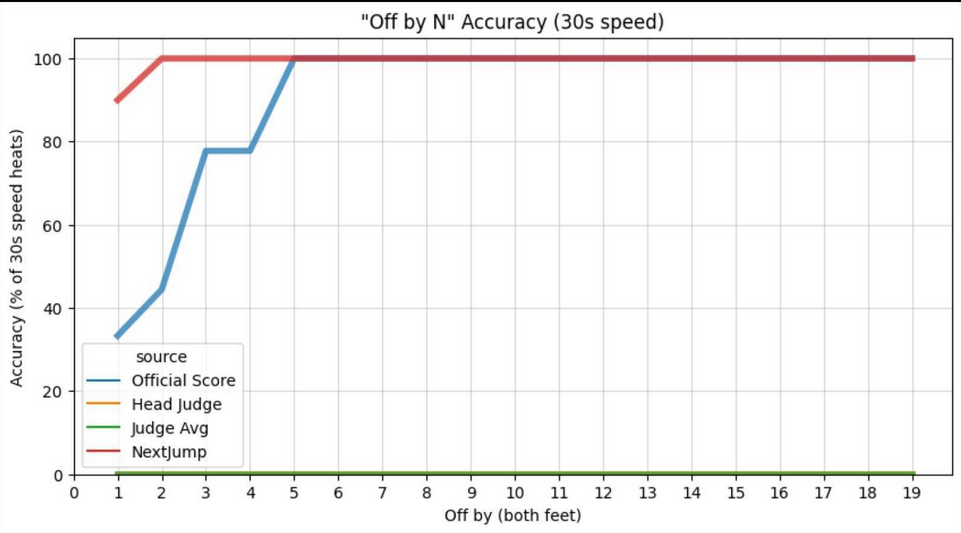
\includegraphics[width=0.95\linewidth]{nextjump-off-by-feet}
    \caption[nextjump-results]{Comparison of avg scores given to a jumper, compared to the effective score. Results are from 2024 AMJRF nationals.}
    \label{proposal-fig:nextjump-off-by-feet}
\end{figure}

\begin{figure}
    \centering
    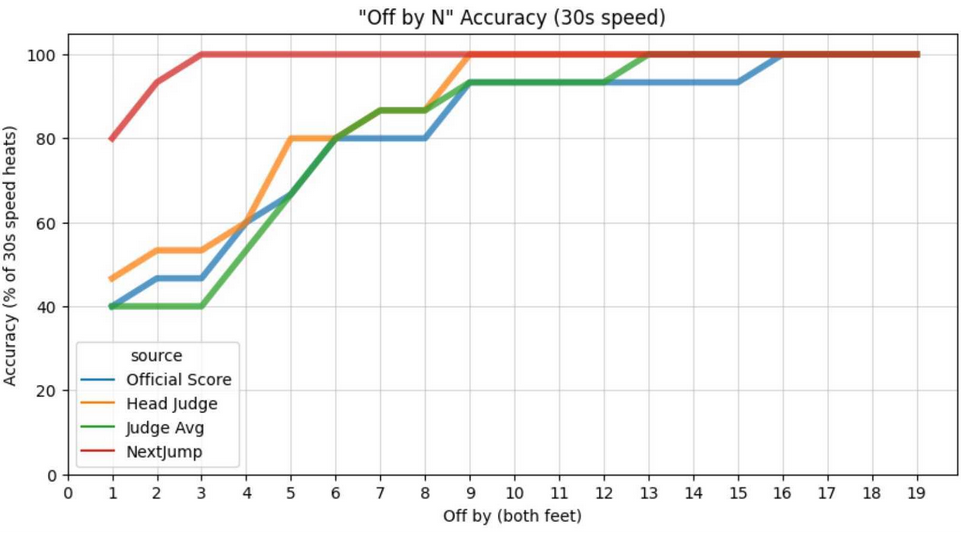
\includegraphics[width=0.95\linewidth]{nextjump-off-by-feet-judges}
    \caption[nextjump-results-multi]{Comparison of avg scores given to a jumper, compared to the effective score. Results are from 2024 AMJRF nationals.}
    \label{proposal-fig:nextjump-off-by-feet-judges}
\end{figure}

As of august 2023, \href{https://nextjump.app/}{NextJump} tested their AI-speed-counter on the world competition acquiring, really accurate results, see fig \ref{proposal-fig:nextjump-off-by-feet} \& \ref{proposal-fig:nextjump-off-by-feet-judges}. They found that 10 hours was sufficient for a single event (e.g. just single rope speed) but to count all kinds of events more (diverse) data is needed\footnote{The current dataset entails 36h video material}. Using this as a base/guidance, the likelihood to succeed implementing skill-recognition in freestyles grows.
When skills are recognized, they can be mapped to their corresponding level and summed up to achieve the total score of a freestyle.


\subsection{HAR general progress}

% TODO : find paper, reference to come to steps or use pareek again?
\textcite{Pareek_2020} did some research about the recent updates in human activity recognition, which mainly gave form to the following general approach.

As jumpers can stand everywhere in a field\footnote{A field is generally 12x12 or 15x15 meters}, locating and cropping athletes can improve the segmentation model\footnote{If time allows it, the final model can be compared with or without localization}. When the skippers are centered, action segmentation can be performed. This allows predicting skills on newly recorded videos, without needing to cut out the different skills. Finally predicting the skill, which can be broken down into multiple, parallel runnable sections.

\begin{enumerate}
    \item Jumper localization
    \item Action segmentation, start/end of skill
    \item Predict the effective skill
        \begin{enumerate}
            \item Predicting the level
            \item Predict skill (power/gymnestic - pushup, split, cartwheel)
            \item Predict turner involvement (cross, EB, TS)
            \item Predict multiple (single, double, triple)
        \end{enumerate}
\end{enumerate}

\subsection{Jumper localization}
\label{proposal-subsec:jumper localization}

Many research towards image recognition has been done \autocite{Zou_2023}. The best models mostly utilize Convolutional Neural Networks pertaining spacial information in the image \autocite{Zaidi_2021}. In their paper, they compare some recent models for object detection such as YOLO(v4), CenterNet, SSD, EfficientDet-D2, each using some backbone architecture like VGG-16, AlexNet, GoogleNet or lightweight models such as ShuffleNet or MobileNet (all using CNN's). Some of them being real-time models (fps > 30).
The goal of localizing the jumper is to center the athletes in the middle of the screen/video. \textcite{Bharadiya_2023} elaborates that the position of objects in images doesn't really matter, but their are no clear statements about the size of objects. It could be that a jumper takes up 80 percent of the screen, while moments later he moved backwards and only takes up 30 percent of the video. Instincts tell us that centered and scaled data will work better later.

One of these models can be taken as a base, using transfer learning\footnote{Concept transfer learning explained in \autocite{Bharadiya_2023}} to fine-tune the results to localize the jumper.

To improve localization, video object segmentation or video instance segmentation can be used. \textcite{Gao_2022} lists some object segmentation models, like SwiftNet \textcite{Wang_2021} using ResNet18 as good and quick model.
Other possibilities would be Cutie \autocite{Cheng_2023}, DensePose (see fig [\ref{proposal-fig:srwrap}, \ref{proposal-fig:srwrapdense}]) \autocite{Guler_2018}

\begin{figure}
    \centering
    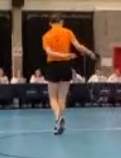
\includegraphics[width=0.3\linewidth]{sr}
    \caption{Jumper wrapping the rope, SR}
    \label{proposal-fig:srwrap}
\end{figure}

\begin{figure}
    \centering
    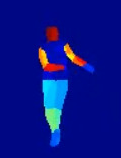
\includegraphics[width=0.3\linewidth]{sr-dense}
    \caption{Jumper wrapping the rope, denseposed}
    \label{proposal-fig:srwrapdense}
\end{figure}

Densepose seems to be able to give the bounding boxes of the main poses detected. Perhaps just a convex hull and some padding will be enough for smart cropping and training a network from scratch is not needed.
However, a local tryout (without boxes) was rather slow, 1.2 fps on GPU within a Docker container, on a laptop.
As jumpers don’t move that much most of the time, skipping some frames and smoothing out the prediction over the rest of the sequence or decreasing the amount of skipped frames when movement is detected, can speed up the localization.

Even when Densepose isn’t used, smoothing can still be applied to the guessed box as a video is basically a sequence of images.

\subsection{Video action segmentation}

When the athletes are cropped, videos need to be split\footnote{Not real/physical splits, but rather labels/annotations for where to split} in (sub)skills, because splitting new videos manually takes to much time and is impractical on competitions. A model like LTContext \textcite{Jiaming_2023} or others\footnote{Using sources like \href{https://paperswithcode.com/task/action-segmentation}{paperswithcode/action-segmentation}} would be appropriate.
Just like the localization, denseposing, extracting poses, foreground, background\dots would improve the segmentation.

The model for generating skill snapshots will
be useful for judging and subsequently labeling
data. Rather than replaying the video, judges can
just sequentially go through each trick one at a
time to assign, annotate or validate the predicted
skill.

\subsection{Skill recognition}
\label{proposal-subsec:skill-recognition}

The final step would be to recognize the total skill in a freestyle video.
\textcite{Yin_2024} did a general HAR survey, also focused on team sports in which they describe the evolution from normal CNN architectures, to recurrent neural networks for time sequences, remembering context, like the Long Short Term Memory model (LSTM). Then combining CNN output into LSTM or even implementing a convolutional filter in the memory cell \autocite{Shi_2015}.

\textcite{Wang_2019} investigated an improvement for current convolutional or recurrent models. They found that LSTM memory cells were too simple to contain higher-order complexities. As a result, they designed a memory in memory component, to replace the previous cell, which could predict actions on complexer data sets. This quickly formed the name Memory in Memory, MIM. Later, \textcite{Lin_2020} used a self-attention memory cell inside the convLSTM that can memorize global aspects in time and space. With about 35\% the number of parameters compared to Wang's MIM-model, SAM achieved a similar score as on the moving MNIST dataset, but faster. Although the focus of these papers was predicting future actions, the output can be transformed into a classification model, rather than a prediction model.

Another approach would be using transformers as a described possibility in \textcite{Yin_2024}, namely ViT-TAD model by \textcite{Yang_2023}, Swin transformer \textcite{Liu_2021} or VideoMAE v2 by \textcite{Wang_2023} seem good options, but further research/try-outs will be required to ensure the transfer models can predict actions.

For reference, NextJump uses a CNN - MobileNetv4, \autocite{MobileNetv4_2024} and a transformer to analyze the full sequence and count. So using the convLSTM, SAM, MobileNet, or a transformer brings us to a better definition or example of what exactly we want to predict.


\subsection{Skill-matrix - complexity \& levels - towards model accuracy}
\label{proposal-subsec:proposal-skillcomplexiteit}

\begin{figure}
    \centering
    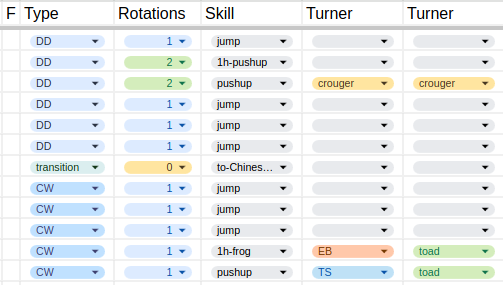
\includegraphics[width=0.95\linewidth]{doubledutch-matrix}
    \caption[skill-matrix-DD]{Representation of a skill-matrix used for Doube Dutch}
    \label{proposal-fig:doubledutch-skill-matrix}
\end{figure}

A basic explanation of skills with some examples was given earlier. In order to recognize all skills, they should be worked out as good as possible. This section explains the composition of the skill-matrix, in order to give a better understanding on the total accuracy of the models later on. As described earlier, skills come with many transitions, take the first skill-matrix representation in figure \ref{proposal-fig:doubledutch-skill-matrix} to better understand skills and transitions.

\textbf{Type:} You have four styles of turning in double dutch; the normal way or double dutch (DD), reversing the rope rotation, sort of like backwards called irish dutch (irish), the chinese way of turning, chinese wheel (CW) or only using one rope or the two combined as a single rope, called single dutch or one rope.

\textbf{Rotations:} The amount of ropes passing underneath the athlete in one jump.

\textbf{Turner:} There are two turners, so two columns, where each turner can execute a turner involvement. Examples are EB, toad or crouger. The cross is in most cases performed by both turners, otherwise the ropes are tangled.

\textbf{Skills:} Mostly powers or gymnastics, but could also be footwork \footnote{Footwork will not be further specified in this paper}. Further distinction or organizing can happen as variation and transitions of powers and gymnastics exists. A recap of different skills would be: pushups, splits, crabs, frogs, swift, cartwheel, salto, webster, suicide, handsprings, round offs \dots % TODO : refer pictures, examples of skills in attachment.
Depending on the exact power or gymnastic, certain characteristics or transitions could be applied:

\begin{itemize}
    \item one handed
    \item one or two feet push-off (e.g. frog vs high frog, salto vs webster, suicide one vs two legged push-off)
    \item turntable \footnote{On way of turning your bodyposition, can be done per quarter e.g. quarter turntable push-up}
    \item full body rotation \footnote{Other way of turning your body, requires full turns}
    \item consecutive \footnote{Consecutive handstands are considered harder and thus get you extra points, not the case with push-up}, e.g. frog after frog
\end{itemize}

Applying these transitions, characteristics allows for more variation, which gets you more points. Repeated skills doesn't get you points. Repetitions are only defined by the skills in the ropes, the speed of the rope (rotations) and the type of turning \footnote{No difference will be made between irish turning and double dutch. Also, only the first skill in single dutch counts}.

\medskip

The skill-matrix is subject to change over time, initial skills not fitting the matrix will be left out for the MVP. Other than skills, jumpers and turners can switch with each other, most of these are also omitted in the MVP.
Each column in the skill-matrix-example 5 can only contain one answer, for which softmax can be used, while between multiple columns, no relation is required and can be predicted separately. This can be solved using a multi-branch output as described in by \autocite{Coulibaly_2022}). This can result in a guessed skill being partially correct, e.g. turner correct, but wrong rotational amount.

On another note, \textcite{Guo_2017} explain that softmax isn't always a good indicator of confidence. They mention that when a model has good calibration, the accuracy should align with the confidence of the prediction. E.g. when you predict a skill has 80\% chance being a push-up, then this prediction or 80\% of the predicted push-ups should be correct. Predictions using softmax tend to be overconfident.

\subsection{Group activity}

As DD3 is a group activity, problems could arise while trying to detect skills. However, the hypothesis is that a DD3 freestyle always acts as one unit, thus not really requiring much special attention. This could pose a problem when adapting SR to SR2 where two individuals are not exactly one unit. Some further research can be done in models like stagNet \autocite{Qi_2020} to improve, incorporate this idea.

\subsection{Unknown/Unusual skills}
\label{proposal-subsec:literature-unknown-unusual-skills}

Unknown skills or special cases pose a problem. That’s why the skill-matrix needs to defined
in such a way that new combinations can fit the matrix as much as possible and/or in combination with zero-shot learning. (Sort of marking unique skills as ’I don’t know’ so that others new/unique ones will also be marked as ’I don’t know’) Unusual skills on the other hand should be incorporated into the implementation.
Earlier an example was given about knocking 3 times on the door. A more concrete example would be turntables, which are mainly performed using a crab or push-up, but also seen with a frog or a split.
Turntables even have the potential to be combined with a swift. Omitting turntable frogs or splits in the train dataset can test this the ability to perform on unusual skills.

\subsection{Summary literature}
\label{proposal-subsec:summary literature}

The PoC needs to localize the jumper \footnote{which can use fine-tuned pre-trained models}, segment actions, and using labeled splits or guessed ones to predict (sub)skills.
Predicted skills will then be mapped to their corresponding level.

%---------- Methodology -------------------------------------------------------
\section{Methodology}%
\label{proposal-sec:methodoly}

After some more research about transformers and how to apply them for skill recognition and another non-transformer models besides convLSTM \& SAM to predict skills, the build process can start.
Using Canva, a \href{https://www.canva.com/design/DAGVz44QCgc/\_Mr9BrOqwwdy9cf-ieYFVg/edit?utm\_content=DAGVz44QCgc\&utm\_campaign=designshare\&utm\_medium=link2\&utm\_source=sharebutton}{user story map} is created to effectively see which tasks need to be done.

\subsection{General \& label location}

\begin{itemize}
    \item overview videos: navigate, filter, rename
    \item view video info, could have edit
    \item label inappropriate/blurry moments (idea: could be used, rather not)
    \item label passage/empty (livestream/wait) moments (idea: no skills)
    \item label jumper location
    \item Statistics of the general data distribution
\end{itemize}

\subsection{Predict location}

\begin{itemize}
    \item visualize jumpoer location predictions
    \item edit borders from new predictions
    \item visualize biggest localization mistakes (within video)
    \item visualize biggest localization mistakes (over all videos)
    \item localization model statistics
    \item data augmentation (if needed)
\end{itemize}

\subsection{Label action segments + label skills}

\begin{itemize}
    \item Label video action segment
    \item Loop-replay action segment
    \item Label segmented skills names
    \item mark false skills
    \item skills to level mapper (should have)
    \item search skills by name (could have)
    \item mark execution scale (could have)
    \item skilldistribution statistics (+/- distributionmatrix)
\end{itemize}

\subsection{Predict action segments}

\begin{itemize}
    \item visualize \& compare AI segmented skills
    \item visualize AI segmented skills from new videos (with confidence levels?)
\end{itemize}


\subsection{Predict skills}

\begin{itemize}
    \item model predicts levels (1-8 classes)
    \item model predicts variation element (4/6 classes)
    \item model predicts skill
    \item add judge scores to freestyles
    \item visualize \& compare AI labeled skills \& compare with total (judge)score
    \item validate AI recognized skills \& save as new training input
    \item label AI recognized skills as new or "i don't know"
    \item action segmentation stats
    \item skillrecognition stats
\end{itemize}


\subsection{Bis}

\begin{itemize}
    \item Language
    \item add competition jump order (easy recordings)
    \item stats competition
    \item insert multiple judge systems
\end{itemize}



\subsection{Answering sub-questions}
\label{proposal-subsec:methodology-sub-questions}



Most answers on the research (sub-)questions are woven into the literature, while others need to wait on the proof of concept to be fully answered.
While labeling skills an answer can be given to question \ref{proposal-subsubsec:intro-question-acceptable-results} acceptable results. The effective usage of models and architectures \ref{proposal-subsubsec:intro-question-earlier-research-guidance} and the educated guess about the data-amount needed to achieve better results \ref{proposal-subsubsec:intro-question-expected-data-to-increase-accuracy} will be answered soon


\subsection{Training \& Hardware}

Working with videos alone requires a lot of resources, let alone training on the data with a normal laptop. It is best to work with one or more GPUs to aid the research process. In between, calculations can be made to estimate how long training sessions will take. This also gives a future reference for other computer vision concepts.


%---------- Verwachte resultaten ----------------------------------------------
\section{Expected results}
\label{proposal-sec:verwachte-resultaten}

Localization of the jumper shouldn't pose an issue. It's would be safe to say that a quick progression towards video action segmentation can be made. Even if segmented actions do not overlap with their actual skills, it's not that hard of a block for the skill recognition part. It would just mean, that skillrecognition can not be applied on new unsegmented videos.
It's expected that SAM will prove to give better results than his base convLSTM model and a transformer probably even better if correctly integrated.

On the long run, it's expected to surpass judges in accuracy.

To answer the questions asked in the introduction a list of unknown or potential answers.

\begin{itemize}
    \item How will the model be built? --> unknown
    \item What would be the main structure of the model? --> unknown
    \item Which human activity recognition examples can be used or altered as the base of the model? --> aligns with modelselection
    \item When are AI-recognitions acceptable to potentially use on competitions? --> when they score equally as good as a judge and can flag or anticipate unknowns.
    \item How much data is expected to increase the accuracy off the Judge. --> we'll know later
    \item How can we use the AI-Judge to improve judges? --> correcting/assisting them.
    \item What needs to changed to a working model, to apply it on other judge-sports such as gymnastics, synchronized swimming... --> define a skill-matrix \& data
\end{itemize}


\section{Expected conclusion}%
\label{proposal-sec:conclusion}

The AI-Judge can improve fairness of judging on competitions by annotating skills and, when expanded, giving confidence levels to the skills it predicted. Using AI-Judge, more transparency towards scores can increase competitiveness or enable the public to better understand the scores. Even using the model to display snapshots of freestyles along the predicted skill and confidence score in total.

This AI-Judge can be extended towards other disciplines or different sports like acro, figure skating, gymnastics or dressage, to achieve similar results.

The next steps will be extending freestyle judging into DD4, SR2 and special skills.
